%%%%%%%%%%%%%%%%%%%%%%%%%%%%%%%%%%%%%%%%%%%%%%%%%%%%%%%%%%%%%%%%%%%%%%
% How to use writeLaTeX: 
%
% You edit the source code here on the left, and the preview on the
% right shows you the result within a few seconds.
%
% Bookmark this page and share the URL with your co-authors. They can
% edit at the same time!
%
% You can upload figures, bibliographies, custom classes and
% styles using the files menu.
%
%%%%%%%%%%%%%%%%%%%%%%%%%%%%%%%%%%%%%%%%%%%%%%%%%%%%%%%%%%%%%%%%%%%%%%

\documentclass[12pt]{article}

\usepackage{sbc-template}

\usepackage{graphicx,url}

\usepackage[brazil]{babel}   
\usepackage[utf8]{inputenc}


\sloppy

\title{Instrução Básicas para Construção de Chat BoT}

\author{Luca Ribeiro Schettino Regne\inst{1}}

\address{Ciência da Computação - Pontíficia Universidade Católica de Minas Gerais (PUC-MG)\\
    Unidade Praça da Liberdade -Belo Horizonte -- MG -- Brazil
\nextinstitute
  Department of Computer Science -- University of Durham\\
  Durham, U.K.
\nextinstitute
  Departamento de Sistemas e Computação\\
  Universidade Regional de Blumenal (FURB) -- Blumenau, SC -- Brazil
  \email{lregne@sga.pucminas.br, 1293230@sga.pucminas.br}
}

\begin{document} 

\maketitle

\begin{abstract}
  This meta-paper has with purpose demonstrate practically how developer a simple Chat Bot in Microsot Azure.  
\end{abstract}
     
\begin{resumo} 
  Este meta-artigo tem por objetivo demonstrar de maneira prática como se desenvolver um Chat Bot na Microsoft Azure.
\end{resumo}


\section{Introdução}

Existe uma crescente demanda de atendimentos instântaneos, eficientes e objetivos. Esse fato alinhado à exigência dos clientes, acaba por gerar uma grande sobrecarga sobre as equipes de atendimentos, e consequentemente às empresas que teem dificuldade para suprir tal demanda.

Visando resolver a problemática citada, vemos cada vez mais as empresas investindo em Inteligência Artificial,  mais especificamente em  Chat Bots para complementar sua equipe de suporte e resolver demandas simples e pontuais. Portanto também se torna crescente a necessidade de profissionais da área da computaço com conhecimento no desenvolvimento dessas tecnologias. 
\section{Conceitos Básicos}
A Inteligência Artificial é uma área que se propôe a produzir tecnologias capazes de simular o racioncínio lógico humano, por meio de adapatções e aprendizado de máquina.

O Chat Bot por sua vez é uma dessas tecnologias que por meio das técnincas citadas simula uma conversa com perguntas e respostas pré-programadas que são adaptadas ao contexto no decorrer do diálogo.

\subsection{Microsoft Azure}
Para o desevolvimento da solução usaremos a plataforma de Cloud da Microsoft conhecida como Azure. Por meio dela é possível abstrair grande parte da solução podendo dar enfoque nas especifidades como: possíveis perguntas realizadas e as respostas à serem dadas após um padrão ser identificado.

\subsection{QnA Maker}
Usaremos como solução o QnA Maker que é uma dessas abstrações que implementa grande parte da A.I, fazendo com que não seja necessário nenhum código para uma solução simples.

\begin{figure}[ht]
\centering
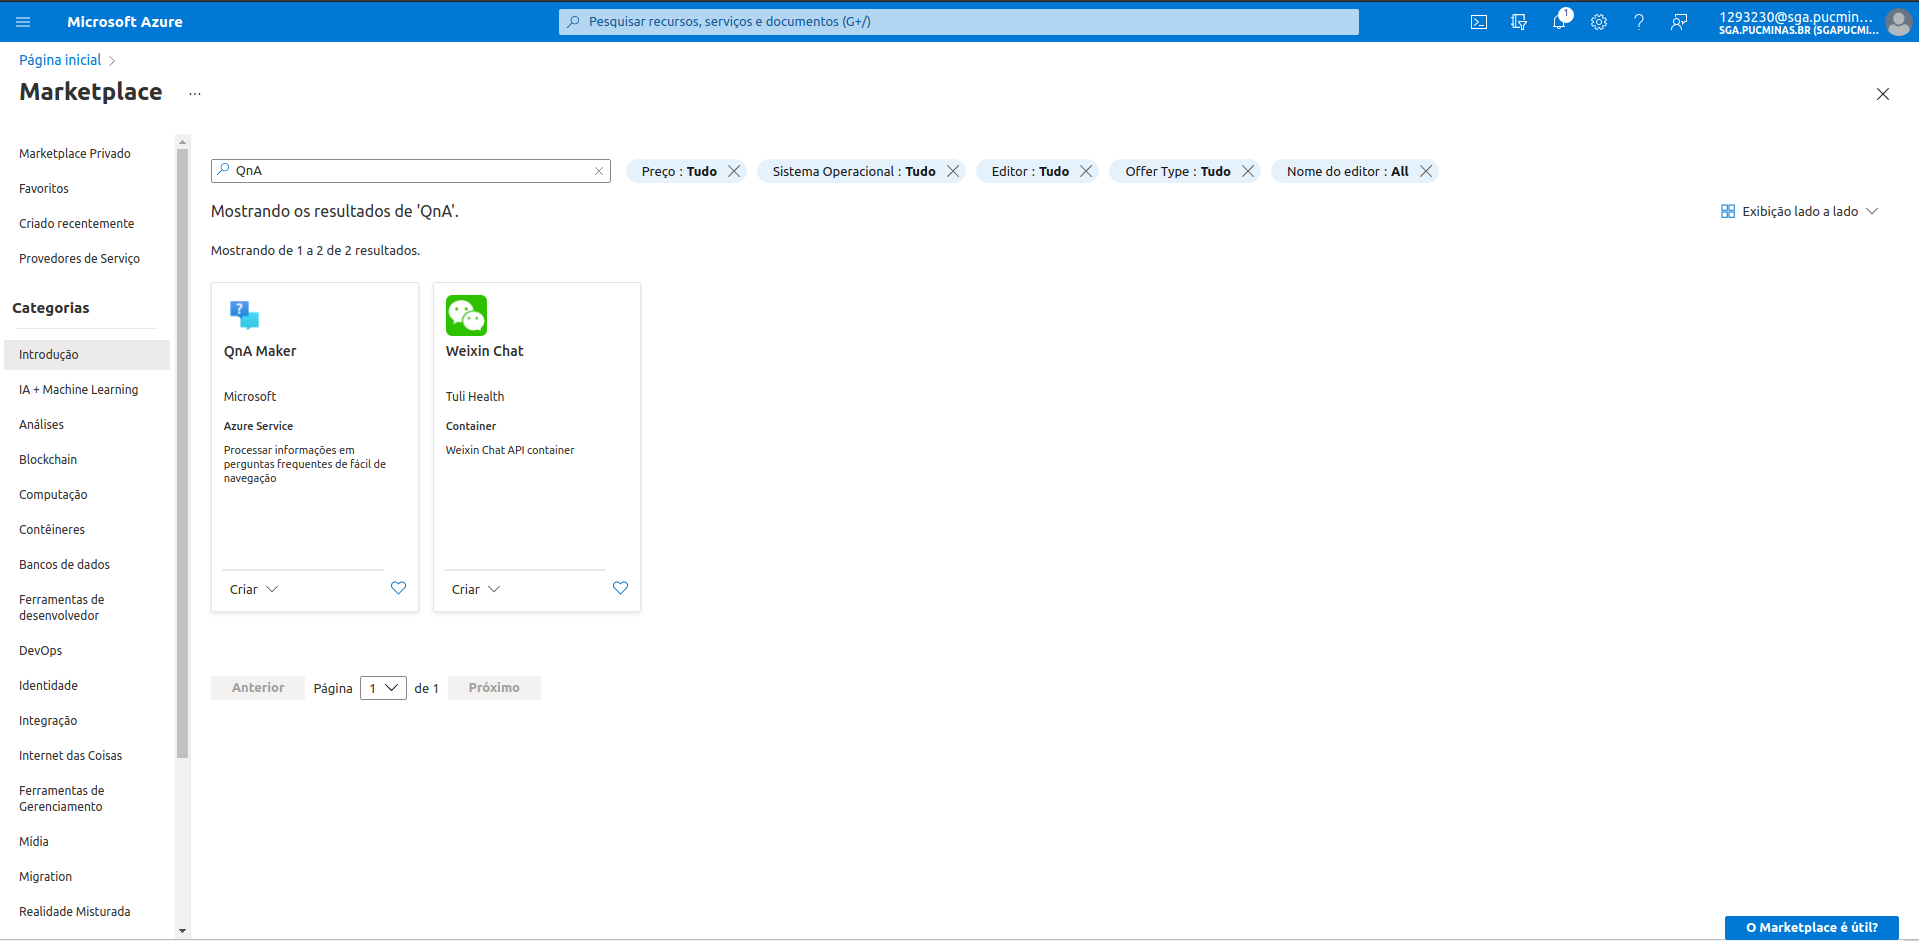
\includegraphics[width=1\textwidth]{images/PortalAzure_QnAMaker.png}
\caption{Busca no Markteplace do Portal Azure por QnA Maker}
\label{fig:PortalAzure_QnAMaker}
\end{figure}

\begin{figure}[ht]
\centering
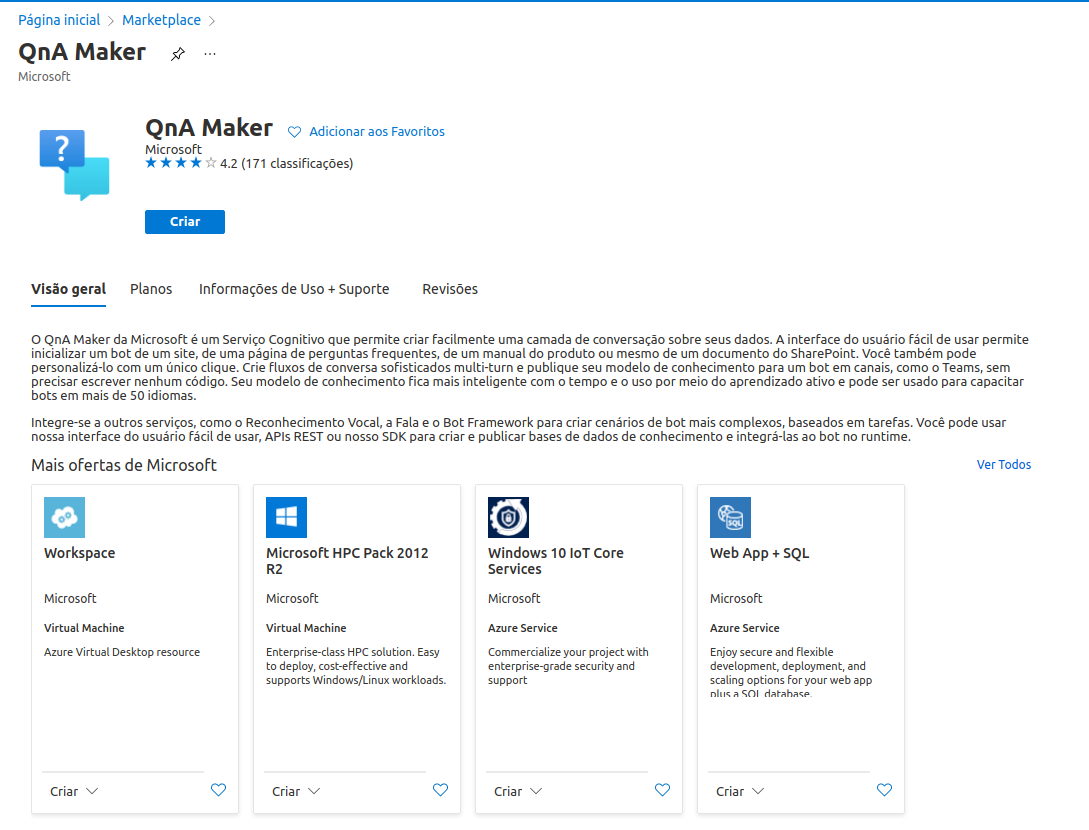
\includegraphics[width=.9\textwidth]{images/QnA_Maker.png}
\caption{QnA Maker}
\label{fig:PortalAzure_QnAMaker}
\end{figure}


\section{Criação do FAQ e Resutaldos }

\begin{figure}[ht]
\centering
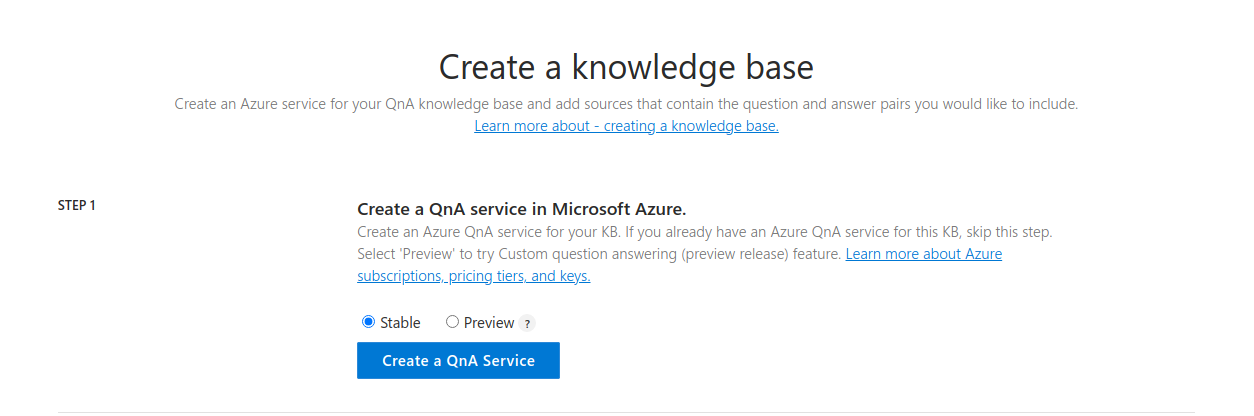
\includegraphics[width=1\textwidth]{images/KnowledgeBase_1.png}
\caption{Etapa 1}
\label{fig:exampleFig1}
\end{figure}

\begin{figure}[ht]
\centering
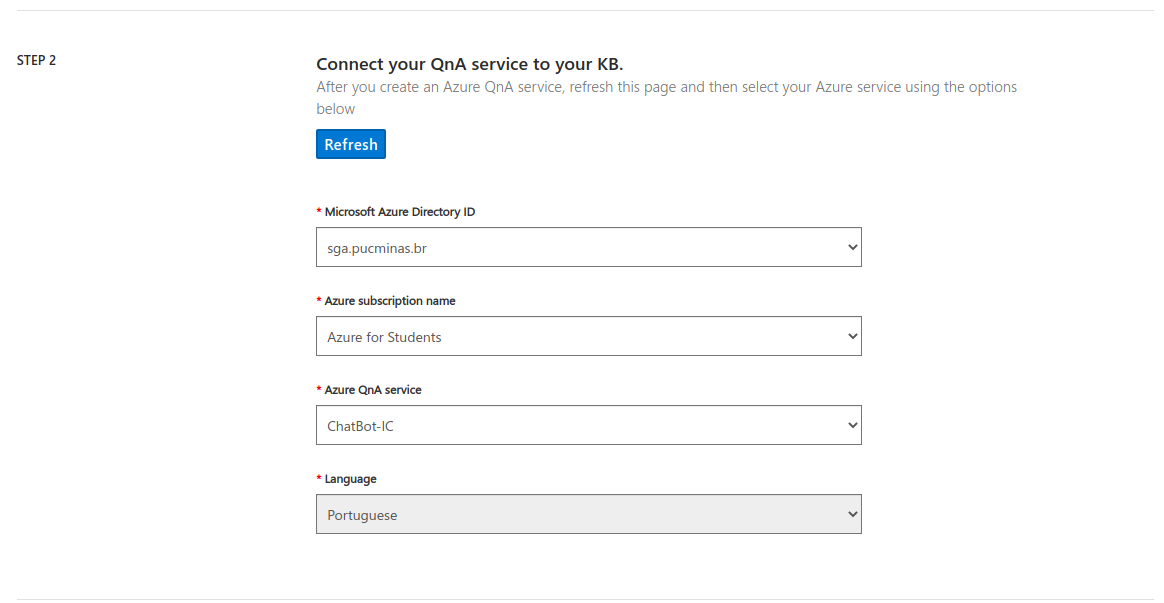
\includegraphics[width=1\textwidth]{images/KnowledgeBase_2.png}
\caption{Etapa 2}
\label{fig:exampleFig1}
\end{figure}

\begin{figure}[ht]
\centering
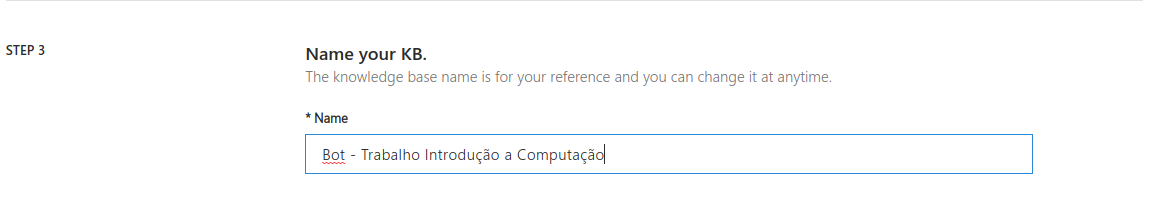
\includegraphics[width=1\textwidth]{images/KnowledgeBase_3.png}
\caption{Etapa 3}
\label{fig:exampleFig1}
\end{figure}

\begin{figure}[ht]
\centering
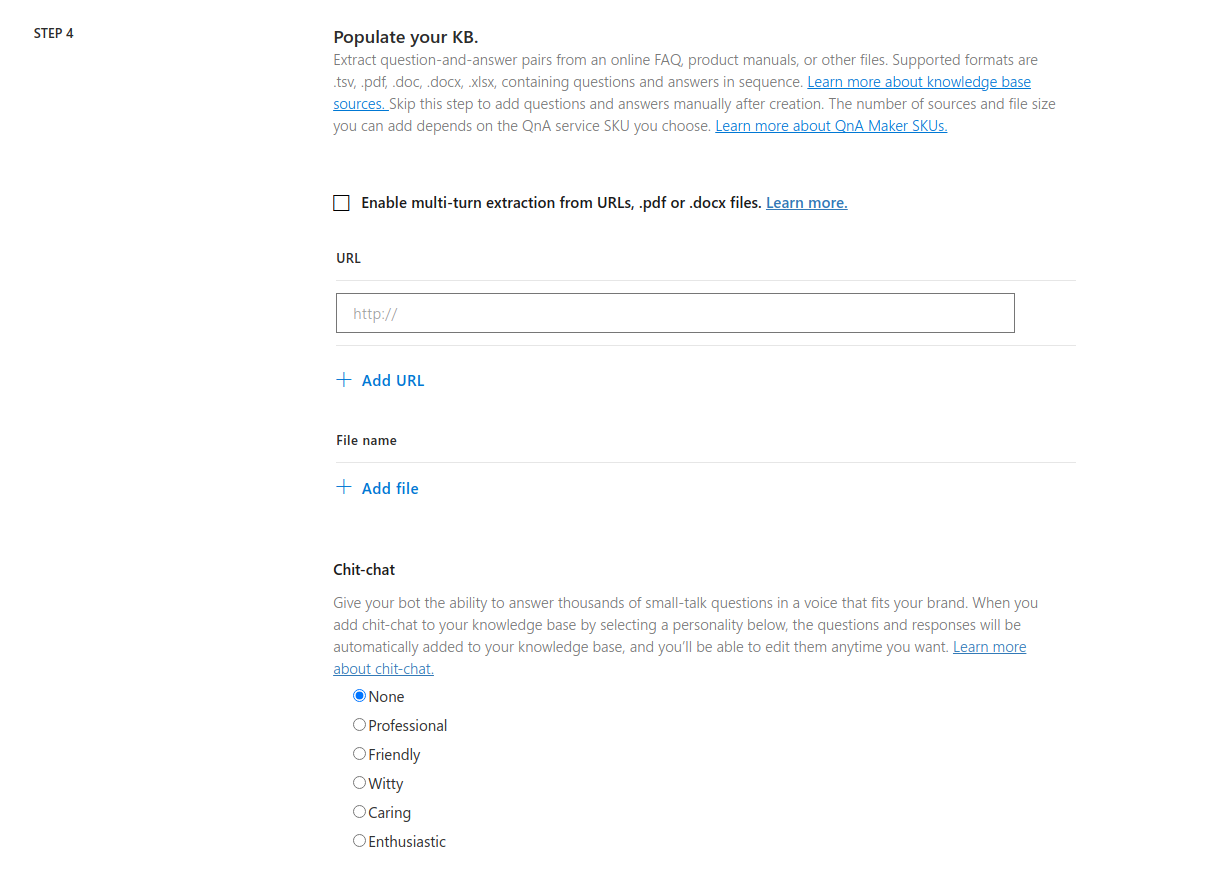
\includegraphics[width=1\textwidth]{images/KnowledgeBase_4.png}
\caption{Etapa 4}
\label{fig:exampleFig1}
\end{figure}

\begin{figure}[ht]
\centering
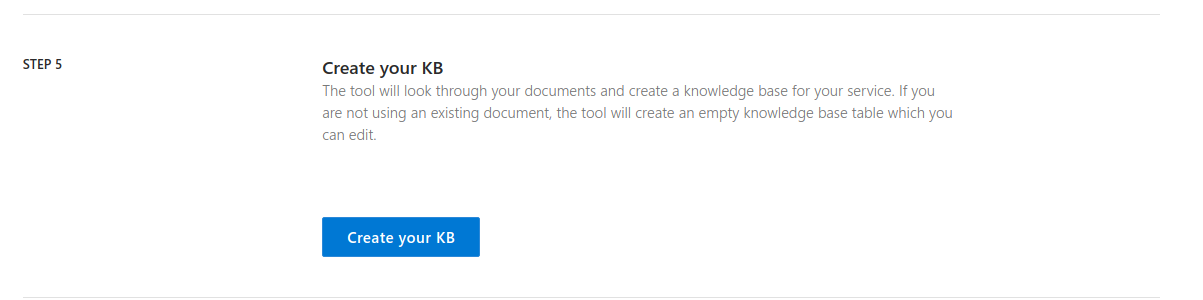
\includegraphics[width=1\textwidth]{images/KnowledgeBase_5.png}
\caption{Etapa 5}
\label{fig:exampleFig1}
\end{figure}

\begin{figure}[ht]
\centering
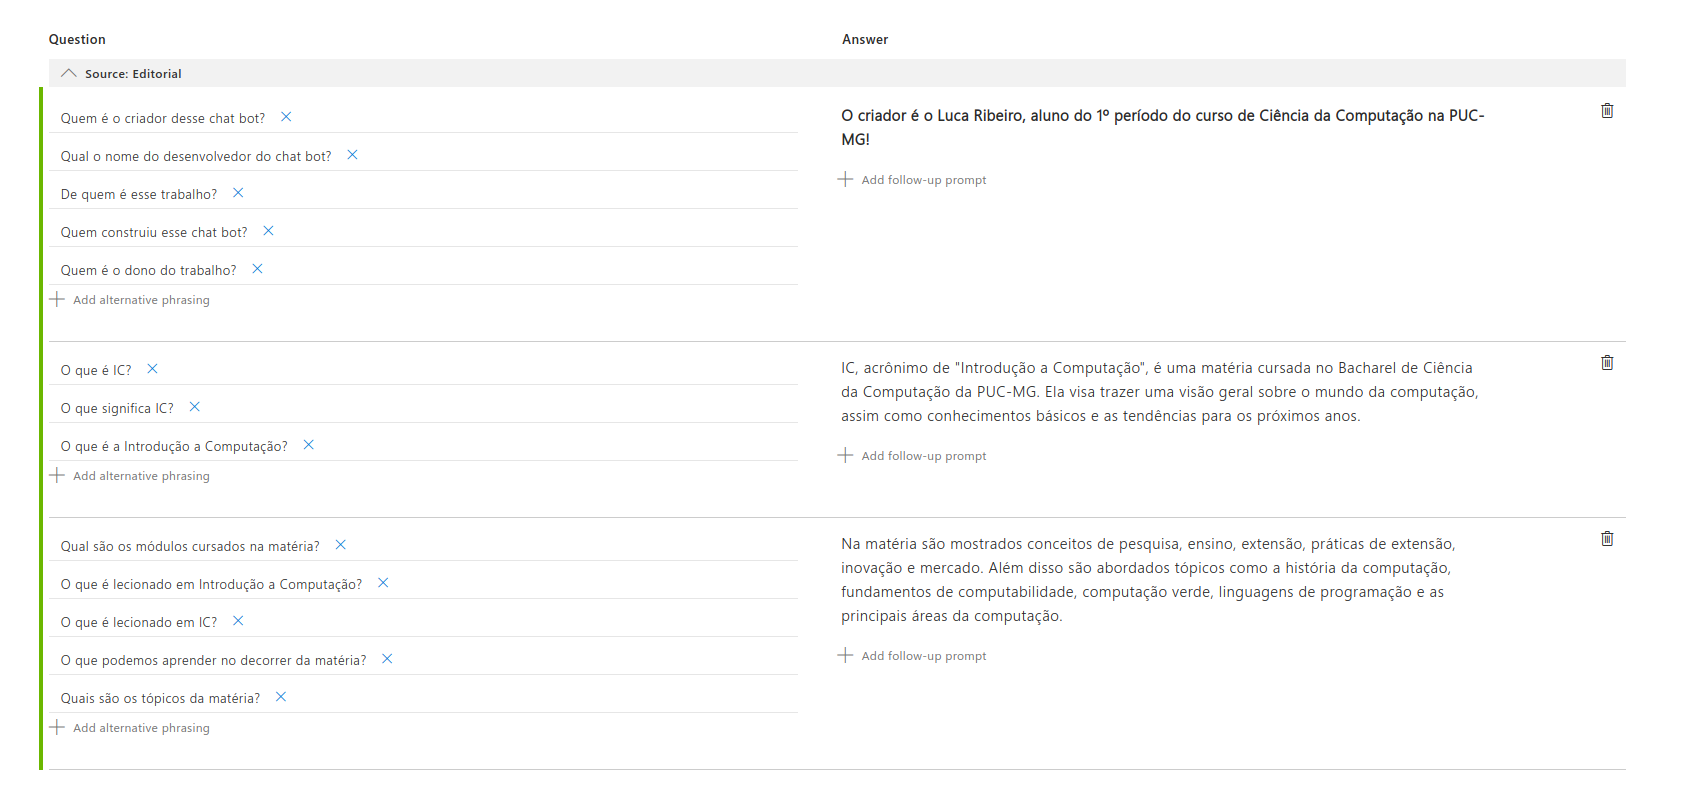
\includegraphics[width=1\textwidth]{images/Perguntas Respostas_1.png}
\caption{Perguntas e Respostas}
\label{fig:exampleFig1}
\end{figure}

\begin{figure}[ht]
\centering
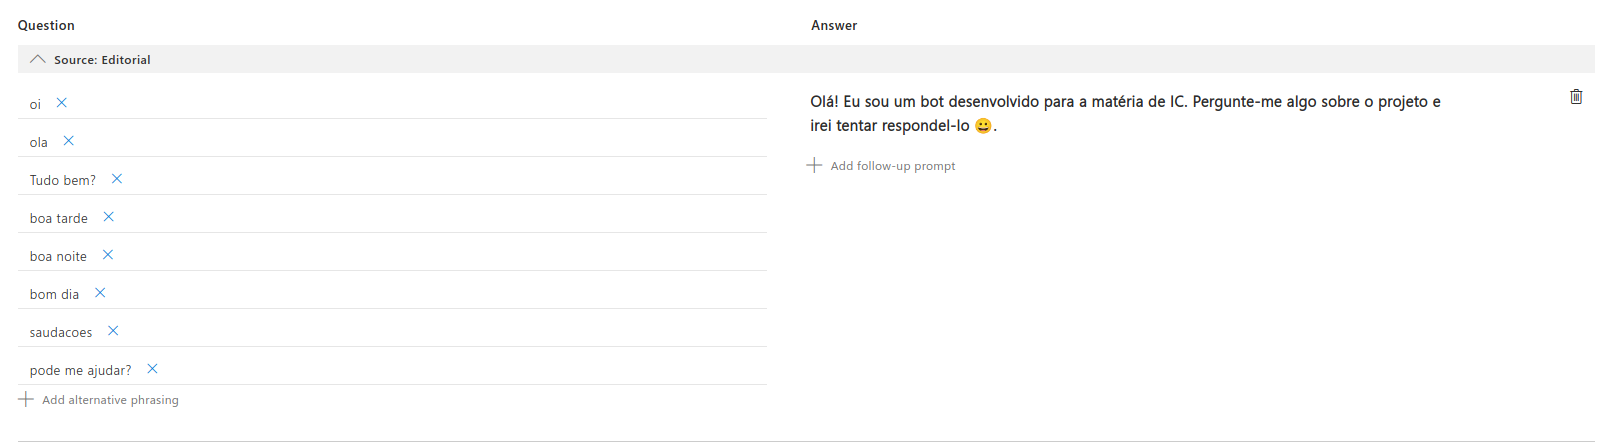
\includegraphics[width=1\textwidth]{images/Perguntas Respostas_2.png}
\caption{Cumprimentos}
\label{fig:exampleFig1}
\end{figure}

\begin{figure}[ht]
\centering
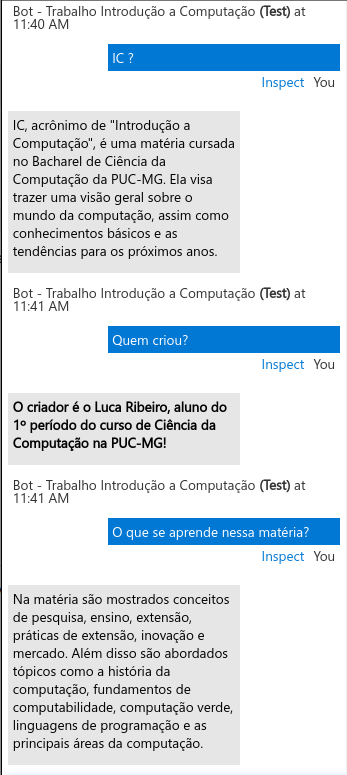
\includegraphics[width=.5\textwidth]{images/ChatBot.png}
\caption{A typical figure}
\label{fig:exampleFig1}
\end{figure}

\end{document}
